\documentclass{standalone}
\usepackage[T1]{fontenc}
\usepackage{xcolor}
\usepackage{tikz, pgf-umlcd, xpatch}
\usepackage{amsmath, amssymb}
\usepackage{gradient-text}

\usetikzlibrary{backgrounds}

\definecolor{background}{HTML}{202020}
\definecolor{umlfillcolor}{HTML}{403f40}
\definecolor{umltextcolor}{HTML}{ffffff}
\definecolor{umldrawcolor}{HTML}{f20ae7}
\definecolor{textcolor}{HTML}{ffffff}

\definecolor{void}{HTML}{939393}
\definecolor{private}{HTML}{ff8000}
\definecolor{protected}{HTML}{80c000}
\definecolor{public}{HTML}{00ff00}

\renewcommand{\umlfillcolor}{umlfillcolor}
\renewcommand{\umltextcolor}{umltextcolor}
\renewcommand{\umldrawcolor}{umldrawcolor}

\color[HTML]{ffffff}

\newcommand{\att}[3]{\attribute{#1 #2 : #3 \hfill}}
\newcommand{\op}[4]{\operation{#1 #2(#3) : #4 \hfill}}

\newcommand{\pri}{\color{private}- \color{textcolor}}
\newcommand{\pro}{\color{protected}\# \color{textcolor}}
\newcommand{\pub}{\color{public}+ \color{textcolor}}
\newcommand{\void}{\color{void}void \color{textcolor}}
\newcommand{\variadic}{Args...}
\newcommand{\cstring}{\color[HTML]{079bdb}C-String\color{textcolor}}
\newcommand{\arr}[2]{#1\color{yellow}[\color{textcolor}#2\color{yellow}]\color{textcolor}}
\newcommand{\virtual}[1]{\color[HTML]{f707bf}#1\color{textcolor}}

\begin{document}
    
    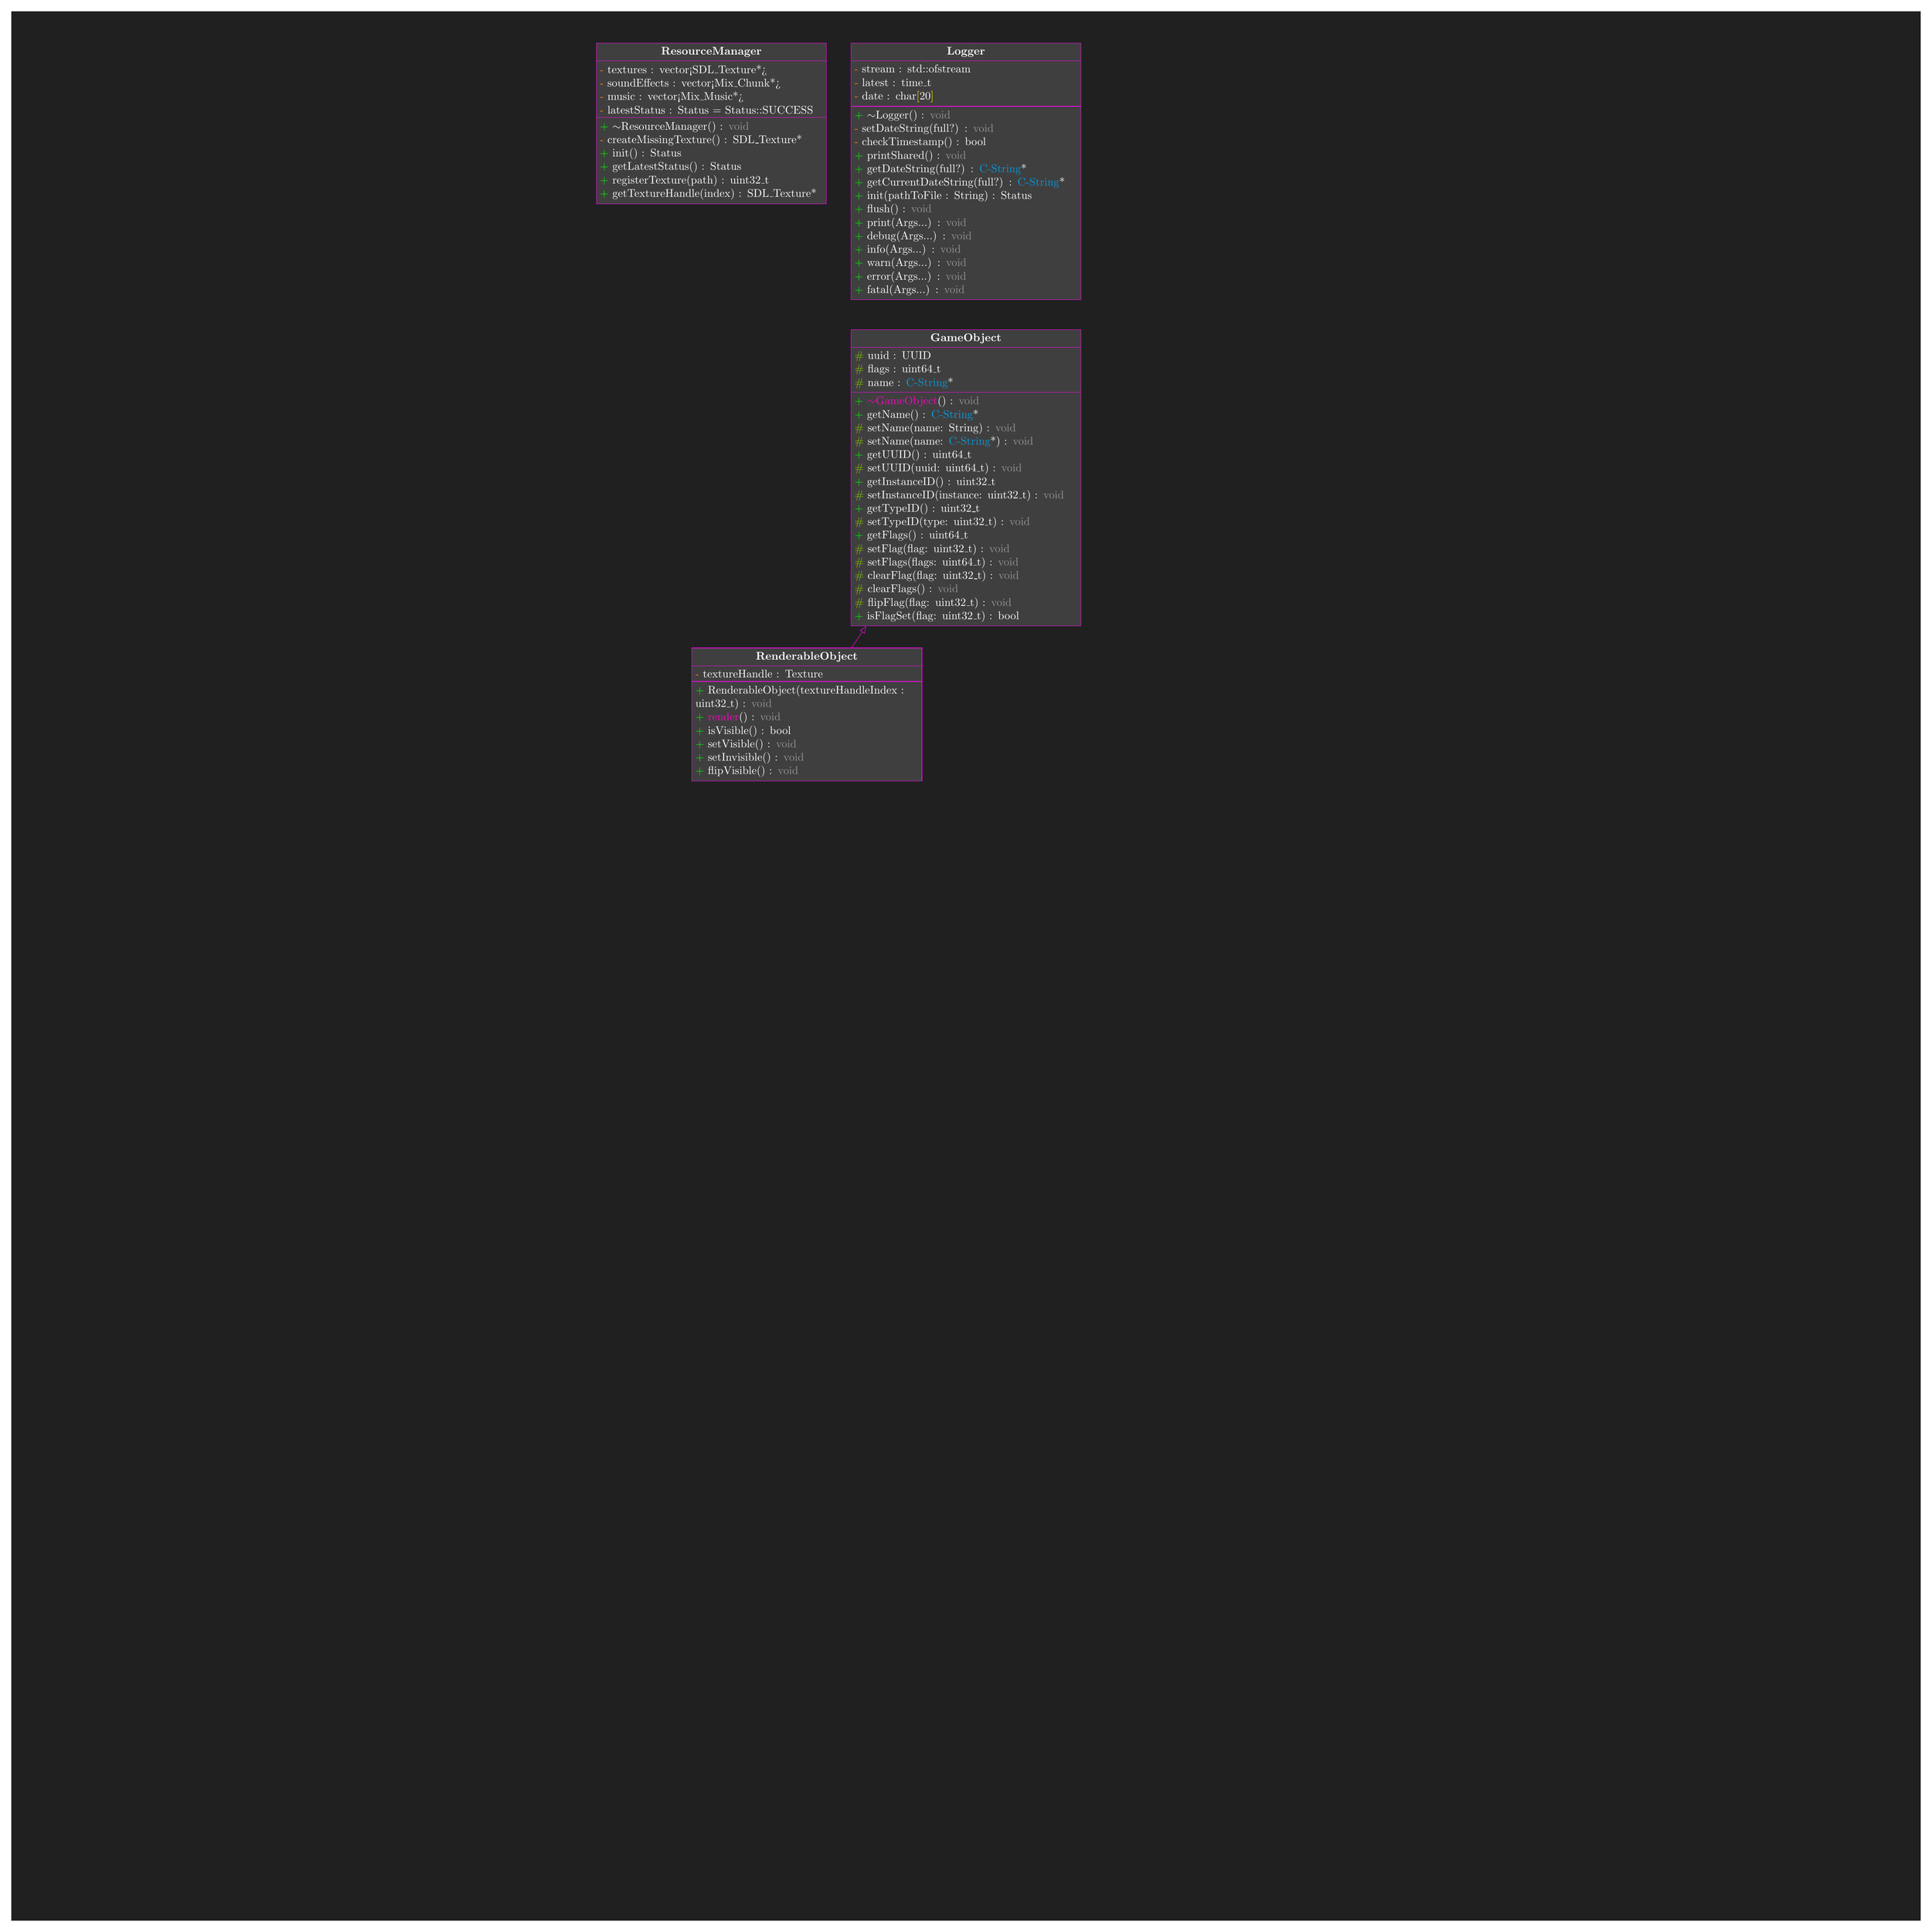
\begin{tikzpicture}
        
        \begin{scope}[on background layer={color=background}] 
            \fill (-30,-30) rectangle (30,30);
        \end{scope}
        \begin{class}[text width=7cm]{Logger}{0, 29}
            \att{\pri}{stream}{std::ofstream}
            \att{\pri}{latest}{time\_t}
            \att{\pri}{date}{\arr{char}{20}}

            \op{\pub}{$\sim$Logger}{}{\void}
            \op{\pri}{setDateString}{full?}{\void}
            \op{\pri}{checkTimestamp}{}{bool}            
            \op{\pub}{printShared}{}{\void}
            \op{\pub}{getDateString}{full?}{\cstring*}
            \op{\pub}{getCurrentDateString}{full?}{\cstring*}
            \op{\pub}{init}{pathToFile : String}{Status}
            \op{\pub}{flush}{}{\void}
            \op{\pub}{print}{\variadic}{\void}
            \op{\pub}{debug}{\variadic}{\void}
            \op{\pub}{info}{\variadic}{\void}
            \op{\pub}{warn}{\variadic}{\void}
            \op{\pub}{error}{\variadic}{\void}
            \op{\pub}{fatal}{\variadic}{\void}
        \end{class}
        \begin{class}[text width=7cm]{ResourceManager}{-8, 29}
            \att{\pri}{textures}{vector<SDL\_Texture*>}
            \att{\pri}{soundEffects}{vector<Mix\_Chunk*>}
            \att{\pri}{music}{vector<Mix\_Music*>}
            \att{\pri}{latestStatus}{Status = Status::SUCCESS}
            
            \op{\pub}{$\sim$ResourceManager}{}{\void}
            \op{\pri}{createMissingTexture}{}{SDL\_Texture*}
            \op{\pub}{init}{}{Status}
            \op{\pub}{getLatestStatus}{}{Status}
            \op{\pub}{registerTexture}{path}{uint32\_t}
            \op{\pub}{getTextureHandle}{index}{SDL\_Texture*}
        \end{class}
        \begin{class}[text width=7cm]{GameObject}{0, 20}
            \att{\pro}{uuid}{UUID}
            \att{\pro}{flags}{uint64\_t}
            \att{\pro}{name}{\cstring*}

            \op{\pub}{\virtual{$\sim$GameObject}}{}{\void}
            \op{\pub}{getName}{}{\cstring*}
            \op{\pro}{setName}{name: String}{\void}
            \op{\pro}{setName}{name: \cstring*}{\void}
            \op{\pub}{getUUID}{}{uint64\_t}
            \op{\pro}{setUUID}{uuid: uint64\_t}{\void}
            \op{\pub}{getInstanceID}{}{uint32\_t}
            \op{\pro}{setInstanceID}{instance: uint32\_t}{\void}
            \op{\pub}{getTypeID}{}{uint32\_t}
            \op{\pro}{setTypeID}{type: uint32\_t}{\void}
            \op{\pub}{getFlags}{}{uint64\_t}
            \op{\pro}{setFlag}{flag: uint32\_t}{\void}
            \op{\pro}{setFlags}{flags: uint64\_t}{\void}
            \op{\pro}{clearFlag}{flag: uint32\_t}{\void}
            \op{\pro}{clearFlags}{}{\void}
            \op{\pro}{flipFlag}{flag: uint32\_t}{\void}
            \op{\pub}{isFlagSet}{flag: uint32\_t}{bool}
        \end{class}

        \begin{class}[text width=7cm]{RenderableObject}{-5, 10}
            \inherit{GameObject}
            \att{\pri}{textureHandle}{Texture}

            \op{\pub}{RenderableObject}{textureHandleIndex : uint32\_t}{\void}
            \op{\pub}{\virtual{render}}{}{\void}
            \op{\pub}{isVisible}{}{bool}
            \op{\pub}{setVisible}{}{\void}
            \op{\pub}{setInvisible}{}{\void}
            \op{\pub}{flipVisible}{}{\void}
        \end{class}

        
    \end{tikzpicture}
\end{document}